\chapter{Introduction}\label{c:Introduction}
\section{Overview of this thesis}
The study of cross-linguistic functional categories such as evidentiality, egophoricity, epistemic modality, engagement, and mirativity is a growing field in linguistics, seeing a huge rise in number of publications over the forty years since \citeA{ChafeNichols1986} made a case for evidentiality as a cross-linguistic category. This thesis provides a typological overview of these categories within the \lfam\ language family, a language family showing widespread epistemic marking and home to many of the languages which informed our early understanding of these categories. It uses published data and analyses of epistemic marking in 67 \lfam\ languages,\footnote{A full list is given in \appref{a:TableOfLanguages}} and original data and analysis of one language, to draw up an initial typological description of this marking in the family. This foundation is then used to establish some broader theoretical conclusions about epistemic marking in the \lfam\ family and cross-linguistically. It argues for a cross-linguistically valid supercategory of epistemic marking (introduced in \ref{s:Intro:Thesis} below) linking these traditionally similar-but-separate functional categories visible throughout the \lfam\ family both functionally and formally, and presents this category of epistemic marking as better able to account for some features of these grammatical systems described in \lfam\ languages.

This thesis is divided into seven chapters. This first chapter provides an overview of the thesis and its argument, followed by an overview of the literature and relevant definitions on important and relevant concepts such as epistemic marking, intersubjectivity, and perspective in language in \cref{c:Foundations}. Chapter \ref{c:THOverview} gives an in-depth introduction to the \lfam\ language family, including an overview of the family, the current state of research and description, and the history of linguistic research in the area. Chapter \ref{c:Methods} details the development of a database of summarised descriptions of \lfam\ languages in terms of the selection of languages and data, along with its representation in an accessible and comparable format. Chapter \ref{c:Description} presents an initial description of epistemic marking in \lfam\ languages from the data, providing a number of typological observations in terms of the forms and functions of grammaticalised epistemic marking across the family. Chapter \ref{c:History} uses the substantial amount of typological data now collected to investigate possible pathways for the development of the widespread epistemic marking seen across the \lfam\ family in historical terms, considering both linguistic and extra-linguistic factors such as population contacts through trade or political influence. Chapter \ref{c:Discussion} takes the typological observations in \cref{c:Description}, along with the view of the family established in \cref{c:History}, and draws more in-depth theoretical conclusions about epistemic marking both in \lfam\ languages and more generally. Finally, Chapter \ref{c:Conclusion} concludes with a summary of the arguments and findings presented in the earlier chapters. Two appendices are included. \appref{s:Methods:FieldMethods} describes the fieldwork conducted on the underdescribed language Lhokpu (Subfamily unclear: Bhutan) to fill in a gap in the available data, including a discussion on the field methods and elicitation of epistemic marking, and an early-stages description of the epistemic marking system in the language. \appref{a:TableOfLanguages} provides a table of all languages systematically surveyed as described in \cref{c:Methods}.

In order to ensure better coverage of the \lfam\ family in this survey (discussed further in Section \ref{ss:Methods:RepSample}) and fill in a gap in the available data, as well as to analyse epistemic marking from a primary source and use this experience to better inform the use of secondary analyses, some fieldwork was conducted on the under-described Lhokpu language. Descriptive publication on the language are limited to \citeA{Grollmann2018}, a comparison of a word list and some basic grammatical forms with Dhimal and Toto (Dhimalish: Nepal and India respectively), which did not provide enough detail to include it in the survey. This fieldwork, detailed in Appendix \ref{s:Methods:FieldMethods}, allowed for the language to be included in the survey though its findings are at this stage still very preliminary. It also allowed for an assessment of methodologies in the documentation and description of epistemic forms, and provided better insights into the complexity of epistemic marking in discourse, in part guiding the direction of the investigation and analysis presented in this thesis.

Given the number of languages across the \lfam\ family discussed throughout this thesis, language names will be presented with their subfamily (as per \citeA{VanDriem2014}, see Sections \ref{ss:THOverview:Subfamilies} and \ref{ss:Methods:RepSample} for discussions on the subfamily structure of the family) along with the country in which they are spoken, for example Hyow \cite[Kukish: Myanmar,][]{Zakaria2018}. In cases where a language is not clearly a member of a wider subfamily, it is labelled as either \textit{Internal isolate} if the classification has been determined by substantial research (e.g. Tshangla \cite[Internal isolate: Bhutan,][]{Grollmann2020}) or \textit{Subfamily unclear} if this is due to a lack of research.


\section{Epistemic marking and the \lfam\ family}\label{s:Intro:Thesis}
This thesis argues, most centrally, that epistemic marking appears across the \lfam\ family can be analysed as a single, functionally cohesive, cross-linguistic category subsuming a number of traditional cross-linguistic categories. This epistemic marking supercategory is represented in this thesis as a strategy for the establishment of shared epistemic ground between speech act participants in the context of the speech act across the \lfam\ family, specifically through the coordination of claims over epistemic authority over information. While this core functional motivation appears widespread across the family, there is a great deal of variation in the division of the gradient of epistemic authority into contrastive epistemic bases and the specific contextual factors that condition their use. Despite this wide variation across the family both formally and functionally, epistemic marking in the \lfam\ language regularly exists functionally across the boundaries of traditional descriptive or cross-linguistic categories, with these cross-categorical meanings encoded either within a single form and epistemic base, or by contrastive forms within a single epistemic-marking system.

Language use, especially speech and conversation, necessarily exists in a context rich environment. The speech act participants (being the speaker and addressee(s)) always have some relationship with the proposition under discussion, in the form of knowledge, awareness, and opinions relating the content of the proposition in the context in which it is being spoken. For instance, a speaker has just noticed a small dog across the road, and points it out to their addressee. Here, the speaker is confident in the truth of their statement, as they can see the dog directly, though may perhaps be surprised to have seen it in this given context. These factors form part of the relationship of the speaker to the proposition they are stating. The addressee also will have a contextually dependent relationship to the proposition; for instance, whether or not they had also seen the dog and were already aware of it, whether or not they also find its presence surprising, and whether or not they would be able to see it directly, now it has been brought to their attention. In many languages, these relationships are not directly encoded in the speech act by default, though in some cases, they can also be seen reflected grammatically or lexically either in every speech act or in specific marked contexts. This grammaticalised marking of the relationship between speaker, addressee, and the information at hand (the proposition) is widespread in the \lfam\ family, as has been addressed in a substantial body of literature to date \cites{Aikhenvald2004}{Hill2017}. This thesis argues that this marking, including the cross-linguistic categories of \textsc{evidentiality}, \textsc{epistemic modality}, \textsc{egophoricity}, \textsc{mirativity}, and \textsc{engagement}, can be analysed in \lfam\ languages as forming a coherent functional domain and category, at the very least for comparative purposes. While these are all well-established categories in the literature---introduced in Section \ref{s:Intro:EpistemicIntro} with definitions and literature reviews---their occurrence in \lfam\ languages is characterised by a great deal of overlap in formal and functional terms. In particular, \textsc{mixed systems}, in which a single cohesive system of epistemic marking (such as a single paradigm) reflects meanings across, for instance, evidentiality, engagement, and egophoricity, are widespread. These systems are difficult to analyse without considering these previously more separate cross-linguistic categories under a single umbrella. Previous attempts to account for this in Tibetic and East Bodish languages in particular include \citesA{DeLanceyMirativity1997}{DeLancey2018Evidentiality}{Gawne2017}{HengeveldOlbertz2012}{Hill2012}{Hyslop2014}, though none have done so under the framework of a single, more unified functional category covering the more general meaning of the relationship between speech act participants and the proposition.\footnote{\citeA{Gawne2013} has argued in favour of treating these systems in their own terms, rather than within the existing more siloed frameworks, though does so at a smaller scale, and places Evidentiality and Epistemic Modality within the much larger concept of Modality as opposed to a more specific cross-linguistic category as is being argued here.} Additionally, the functional overlaps between these categories have been explored in more individual terms throughout the literature, presented in Section \ref{ss:Intro:Overlaps}. This thesis proposes this higher order functional domain as marking a broader category of \textsc{epistemic} meaning, in turn being referred to \textsc{epistemic} marking. In reflecting the relationship of both speech act participants (the speaker and addressee) to the speech act itself, an important part of the discussion of epistemic marking then is reference to the perspectives of these two speech act participants. A well-established aspect of this attention to perspective is the shift from a reflection of the perspective of the speaker to that of the addressee when moving from a declarative structure to an interrogative one \cites[242]{Aikhenvald2004}{EgoIntro}, perhaps as a predictable outcome of the pragmatics of conversation \cite{Hill2020}. However, as Chapter \ref{c:Discussion} argues, the reflection of the perspectives of the speaker and addressee is much more complex and pervasive than previous analysis would suggest, and that in fact conversation more generally always involves an assessment by the speaker of their own perspective, along with a projection or assessment of the perspective of their addressee and potentially other individuals such as characters in narratives. 

A further key concept that is referenced throughout the literature on the individual categories listed above, in particular with regards to engagement \cite{EvansBergqvistSanRoque2018a}, is that of epistemic authority. In analysing epistemic marking as a single functional category as presented in this thesis, it becomes clear that the functional contrasts marked within a single system in a language can generally, if not always, be placed on a gradient of how strongly the speaker is claiming authority over the information at hand (or, in cases such as interrogatives, granting said authority to the addressee), as argued specifically for evidentiality by \citeA{Bergqvist2023}. While there is a great deal of variation in the specific factors of context surrounding a given speech act that can influence exactly where boundaries are drawn along this gradient, this trend provides both further support for their grouping as a single functional domain, as well as a useful tool for their analysis, discussed further in Sections \ref{sss:Description:SpeakerNonSpeaker} and \ref{s:Discussion:Mixed}. These characteristics, along with the widespread nature of the marking and the more general tendency for the marking to spread areally \cite{Aikhenvald2004}, suggest a core functional motivation behind the marking of this epistemic meaning of the support of smooth conversation by establishing a shared ground between speech act participants regarding their respective knowledge surrounding a proposition, along with the nature of this knowledge, discussed further in Section \ref{s:Discussion:Motivations}. As will be discussed in more detail, this in line with the work of \citeA{Heritage2012}, which suggests that the perspectives of both speaker and addressee are unavoidable in `social action'. These motivations, however, are tied to the function of the marking, and are by no means restricted to \lfam\ languages or even the grammaticalised forms of epistemic marking under investigation in this thesis; however could be applied more widely to language and conversation in general.

While typological surveys of some of the categories introduced above have been undertaken at a worldwide scale, perhaps most notably \citeA{Aikhenvald2004}, as well as smaller surveys such as \citesA{EvansBergqvistSanRoque2018a}{EvansBergqvistSanRoque2018b}, no large cross-linguistic surveys of epistemic marking more broadly has been conducted within the \lfam\ family. An exception to this is \citeA{Gawne2021}, a typological survey that focussed only on reportative evidential marking across the family. Despite the prevalence of epistemic marking across the \lfam\ family, no survey has been undertaken to take stock of the marking across the family as a whole and to attempt to describe observed variation and trends. As more and more attention is paid to epistemic marking, the lack of such a broad investigative overview will hinder the ability of researchers to place their research on a single language within a much larger typological context, going beyond that of the immediate siblings or neighbours of the language. In undertaking such a survey, this thesis throws a wide net in two areas. Firstly, it develops a database representative of the marking across the entire \lfam\ family. That does not mean that it is surveying every language in the family, a task that is impossible at with the current state of description as described in Section \ref{ss:Description:StateOfDescription} and within the scope of this thesis. Rather, it is sampling across the family as evenly as possible given the current research in order to avoid missing any particularly noteworthy or aberrant cases without knowing in advance where they will be. This sampling is discussed in detail in Section \ref{ss:Methods:RepSample}. Secondly, this thesis is not limited to a single functional element or even traditional epistemic category, as with \citesA{Gawne2021}{Aikhenvald2004} respectively. Rather, it takes a more general view of the functional domain, arguing for an analysis of epistemic marking as a category unto itself as a supercategory over evidentiality, epistemic modality, egophoricity, mirativity, and engagement, and arguing against the analysis of these categories as functionally and theoretically completely separate.

The term ``supercategory'' is used here to refer to a category acting as an umbrella over multiple other categories. An alternative label would be `meta-category', though this seems to suggest that the category of epistemic marking proposed here is not a category in its own right, but only defined as a collection of other categories. Rather, it will be argued in this thesis that the category is on its own fully motivated by a single coherent functional domain acting to coordinate shared epistemic ground between speech act participants. At the same time, it exists over the top of the other, more narrowly defined categories of evidentiality, egophoricity, mirativity, engagement, and epistemic modality, categories which, as is discussed below, appear to be more defined on semantic terms rather than in terms of function or usage.

\chapter{Theoretical foundations}\label{c:Foundations}
\section{Introduction}
This chapter provides some theoretical foundations of concepts that will be used and addressed throughout the thesis, reviewing previous research and definitions to provide a theoretical foundation for its analysis. It introduces and defines the term epistemic marking as a supercategory, encompassing the categories of epistemic modality, evidentiality, egophoricity, mirativity, and engagement (\sref{s:Intro:EpistemicIntro}), the validity of which is argued by this thesis. \sref{s:Intro:Theory} defines and discusses three important theoretical topics upon which conclusions will be drawn; namely, research into perspective-marking, the distinction between proposition and metaproposition, and the terms subjective and intersubjective and their histories.

\sref{s:Intro:Categories} introduces and defines the categories of epistemic modality, evidentiality, egophoricity, mirativity, and engagement, considering the history of research into the concepts and the current state of the literature both within the \lfam\ family and more generally. Finally, \ref{ss:Discussion:SpeechActs} provides a brief foundation into the description of speech acts and the underlying functional content of forms as they are used in discussion in this chapter, specifically presenting two descriptive construals of the process behind the selection of forms. These two construals are not different in any real terms beyond their conceptualisation of the process, allowing for better explanation throughout this chapter.

\section{Definitions and previous research on epistemic marking}\label{s:Intro:EpistemicIntro}
\subsection{Epistemic marking}
Epistemic marking and meaning are growing areas of study in pragmatics, and in linguistics more generally. The term is used here to refer to a number of cross-linguistically observable phenomena in which speakers place themselves, as well as the addressee, in the context of the information they are communicating. That is, it is a function through which the speaker can mark the relationship of themself, the addressee, or both, to the proposition at hand and its content. 

These cross-linguistically observable phenomena, as described by current literature, are \textsc{evidentiality}, a category marking\footnote{All meanings are given here in relation to their usage in assertions, and in a typical sense. It is not uncommon for patterns to vary in interrogative constructions \cite{Aikhenvald2018Intro}.} the speaker's source of information \cite{SanRoque2019Evidentiality}; \textsc{epistemic modality}, marking the confidence or epistemic support from a speaker over a given piece of information \cite{Boye2012}; \textsc{egophoricity}, a category marking personal authority of a speaker over the information being presented \cite{EgoIntro}; \textsc{mirativity}, marking (at least by definition) a speaker's surprise or lack of previous awareness over the information \cite{DeLancey2012}; and \textsc{engagement}, marking the joint ``access'', or awareness of and physical proximity to, the information being presented \cites{EvansBergqvistSanRoque2018a}{EvansBergqvistSanRoque2018b}.

The term \textit{epistemic}, introduced in Section \ref{s:Intro:Thesis} above, is not necessarily a perfect term for this specific set of phenomena, but is the closest fit available. While the term has potentially more restricted meaning in other fields, notably philosophy (see \citeA[15-18]{Boye2012}), it functions suitably as a descriptive term covering the phenomena and meanings under investigation in this thesis. 

As previously established, this project will focus on the related phenomena of evidentiality, epistemic modality, egophoricity, mirativity, and engagement. All of these phenomena clearly exhibit features of either subjectivity, intersubjectivity, or both. However, these terms alone are insufficient to either accurately characterise the categories themselves, or to separate them out from the wider field of (inter)subjectivity. It will also be argued that \textit{intersubjectivity} alone is an inaccurate label by current literature, and a term already burdened with an excess of different meanings. Each of the phenomena have been researched to various extents on their own, as have interactions between pairs of them in specific languages, though no study of all four has been undertaken to date.

\section{Theoretical underpinnings}\label{s:Intro:Theory}
\subsection{Perspective and point-of-view}\label{ss:Intro:PerspPOVDefs}
The terms \textsc{perspective} and \textsc{point-of-view} are used largely interchangeably in this thesis. The terms are used here to refer simply to the possible differences in awareness between individuals in conversation because of their different experiences, knowledge, and current attention. In this sense, the perspective of an individual is a reflection of the state-of-mind of said individual, and is interchangeable with the term point-of-view. This practice is in line with usage in literature such as \citesA{Evans2005View}{Sweetser2012}{Bergqvist2017}. 

An awareness of the role of perspective in language is by no means a recent development. \citeA{Kamio1997} is a foundational piece of literature investigating this, suggesting that a speaker and addressee and their different perspectives can be described in terms of \textit{territories of information}. In this framework, developed by Kamio in his research on Japanese grammar over the preceeding two decades, a given piece of information can be seen as falling in the territory of the speaker or addressee, or somewhere in between. It is on this foundational concept of the unequal authority over knowledge that much of the analysis of this thesis is based. Extensions of this notion in similar terms have been presented more recently; for instance, \citeA{Heritage2012}, who draws a link between Kamio's territories of information and epistemic meaning, particularly in relation to the construction of interrogative meaning beyond simple grammatical interrogative markers. More recently still, \citeA{GonzalezPerez2023} describes a similar concept of \textit{spheres of interest}, further including spatial and attentional factors in the description of the perspectives of the speaker and addressee. Early literature, however, had a tendency to view the reflection of perspective as an ``either/or'' situation, as noted in \citeA{Evans2005View} in his analysis of the marking of multiple perspectives in Australian languages. Here, Evans seeks to prove initially that multiple perspective constructions are present across multiple languages and can be found in all major semantic categories. These constructions allow a speaker to take two perspectives (for example, and likely most relevantly here, speaker and addressee) at the same time, a clear precursor to engagement. Evans characterises the research as a ``premilinary typology'' (p. 93); interestingly, he suggests that multiple perspective constructions in which the speaker is granted a lower level of authority than the second perspective (e.g., you know this but I don't, or some object is near you but not me) are uncommon. Both of these forms are later attested in \citeA{EvansBergqvistSanRoque2018a}. 

To an extent, much of the literature on perspectives, and in particular the representation of multiple perspectives following \citeA{Evans2005View} acted as growing field of study that eventually resulted in the description of \textit{engagement} as a cross-linguistic category in \citesA{EvansBergqvistSanRoque2018a}{EvansBergqvistSanRoque2018b}. This includes the work of Henrik Bergqvist, who wrote first on Kogi (Arwako-Chichan: Colombia) in \citeA{Bergqvist2016Kogi}, then expanded his work on tying perspectives to epistemic marking in \citeA{Bergqvist2017}. While \citeA{Evans2005View} also suggests a separation between his ``multiple perspectives'' and structures such as evidentials and epistemic modals, which he refers to as ``metaperspectives'' (p. 115), \citeA{Bergqvist2017} investigates the crossover between these areas, suggesting that these multiple perspective constructions are, much like evidentiality, also epistemic in nature, referring to the category later called engagement as \textit{complex epistemic perspective}. This subsequently led to the development of engagement is descriptive work such as \citeA{SanRoque2015}, which presents a (later termed) engagement paradigm in Duna (Trans-New-Guinea: Papua New Guinea) and suggests that the marking might work discursively to maintain common ground between speech act participants.

In these cases, reference to multiple perspectives is largely seen as a typologically uncommon and noteworthy construction. \citeA{Sweetser2012} suggests, in part informed by neurological evidence and in part by linguistic evidence from English, that a consideration of multiple perspectives is unavoidable in discourse. This suggestion is further argued in \citeA{Zeman2019} in both discursive and grammatical terms, though here it regards to constructions referencing the perspective of speaker and a narrative character, rather than speaker and addressee. The proposed universality of multiple perspective reference is also argued in Chapter \ref{c:Discussion} of this thesis. 

Beyond \citesA{EvansBergqvistSanRoque2018a}{EvansBergqvistSanRoque2018b}, much of the literature on reflection of perspective, and in particular multiple perspectives and its grammaticalised marking, is specifically framed in terms of engagement, a review of which is given in Section \ref{s:Intro:EngagementIntro} below.

\subsection{Propositions and metapropositions}
\textit{Proposition}, contrasted with \textsc{metaproposition} below, is used to refer to part of the speech act that is ``in-narrative'', or unconcerned with the context of the speaker. By extension, and in line with the use of the term in \citeA[150]{EvansBergqvistSanRoque2018b}, \textsc{metaproposition} refers to second-order information, or information given by the speaker about the proposition, but not actually affecting the proposition itself. The \textsc{information} is the content of the (meta)proposition---that is, the actual semantic content being communicated. This can be seen in \exref{ex:MetapropEnglish}. Here, (a-b) are plain propositions. The addition of the adverbial construction ``on foot'' changes the meaning of the proposition itself in that it changes (or specifies) the actual event being described. Example (c), however, shows the same proposition, with a metaproposition ``I saw that'' providing information about the speaker's relationship to the proposition, but not causing any changes to the information in the proposition itself (i.e. the narrative that he went to the shops remains unchanged).

\begin{exe}
\ex\label{ex:MetapropEnglish}
\begin{xlist}
\ex He went to the shops.
\ex He went to the shops on foot.
\ex I saw that \{He went to the shops.\}\label{ex:MetapropEnglish:c}
\end{xlist}
\end{exe}

When used in assertions, the categories introduced above mark metapropositional information from the speaker's point-of-view (e.g. \exref{ex:MetapropEnglish:c}. Its metapropositional meaning could be encoded through evidential markers in languages with such marking). However, this is not necessarily always the case, as will be discussed in more detail in Sections \ref{s:Intro:EvidentialityIntro}-\ref{s:Intro:EngagementIntro} below. As a result of this potential shifting of reference, the term \textsc{origo} is used in this thesis to refer to the perspective from which the metapropositional information is being presented, following \citeA{Garrett2001}\footnote{Garrett attributes this term to the work of Karl Bühler, who in turn borrows it from its usage to refer to the centre point of the Cartesian plane \cite{Buehler1965}.} and discussed in detail in Section \ref{ss:Discussion:Origo}. That is, as in \exref{ex:OrigoShift} from Lhasa Tibetan, the egophoric (or personal authority) evidential \textit{yin} (\foreignlanguage{tibetan}{ཡིན}) remains the same in assertions and questions, showing a speaker origo in assertions and an addressee origo in questions. While in \exref{ex:OrigoShift:a} the speaker is stating their own experience, in \exref{ex:OrigoShift:b} the speaker is asking the addressee for their personal authority.

\begin{exe}
\ex\label{ex:OrigoShift}
\begin{xlist}
\ex\label{ex:OrigoShift:a} 
\gll nga bod=pa \textbf{yin} \\ 
1sg Tibetan \textbf{be.\textsc{ego}} \\
\glt `I am Tibetan.' (Personal Authority Evidential/Egophoric, Speaker-Origo)
\ex\label{ex:OrigoShift:b} 
\gll khyed=rang bod=pa \textbf{yin=pas} \\
2sg Tibetan \textbf{be.\textsc{ego}-\textsc{interrogative}} \\
\glt `Are you Tibetan?' (Personal Authority Evidential/Egophoric, Addressee-Origo)
\end{xlist}
Lhasa Tibetan \cite[Tibetic: PRC,][394]{DeLancey2017Tibetan}, function/origo labelling mine
\end{exe}

\subsection{Subjectivity and Intersubjectivity}
The concept of intersubjectivity is, at least in its development, a theoretical extension of research into \textit{subjectivity}, examining the linguistic devices that highlight the speaker as an agentive entity and allow the speaker to orient themselves within the context of the speech act. These are the methods through which speakers can convey their own perspective in addition to the ``objective'', propositional component of meaning \cite{Finegan1995}. At a narrower level of focus, however, the term \textit{subjectivity} is used for a number of different purposes and varied analytical frameworks. These disparate uses of the term are mentioned as early as \citeA{Finegan1995}, who establishes two key schools of usage. The first, developed by \citeA{Lyons1982}, fits closely with the above description, and has been developed into a field of diachronic study focussing on the development of subjectivity through grammaticalisation by \citeA{Traugott1995}. The other school discussed by \citeA{Finegan1995} is one introduced by \citeA{Langacker1985}, approaching the problem of subjectivity synchronically through a Cognitive Grammar lens, a framework introduced below.
    
If subjectivity is the process through which a speaker can establish their perspective or mindset in speech, \textit{intersubjectivity} refers to strategies through which the speaker can work to coordinate their perspective with the perspective of their interlocutor \cite{Brems2014}.

The multiple frameworks working under the term \textsc{(inter)subjectivity} are still treated as largely independent, being discussed in \citeA{Brems2014} in terms of their attention to intersubjectivity. The Traugott and Cognitive Grammar frameworks are characterised in their current form most succinctly by \citeA{Nuyts2015}, who describes the Cognitive Grammar framework as a binary distinction measuring the speaker's presence in an utterance; that is, whether or not the speaker and the speaker's perspective act as a deictic referent in the utterance. Nuyts provides \exref{ex:LangackerNuyts1} as an example of this binary, in which \exref{ex:LangackerNuyts1:Obj} is objective and \exref{ex:LangackerNuyts1:Subj} is subjective.\footnote{\exref{ex:LangackerNuyts1:Obj} contains no reference to the speaker or their position in the scenario (they may not even be present, or, in the case of a narrative, they may not exist in the same world as Mary) while \exref{ex:LangackerNuyts1:Subj} places the speaker in the scenario.} A more subtle example of this can be seen in \exref{ex:MyLangackerNuyts}, showing the same pattern but without the need for an explicit first person reference due to the implication of the speaker as the deictic centre in the phrase ``across the table''. That is, by introducing a point of comparison without any explicit reference point, the speaker is assumed (`from me').

\begin{exe}
\ex\label{ex:LangackerNuyts1}
\begin{xlist}
\ex Mary is sitting at the table. (Objective)\label{ex:LangackerNuyts1:Obj}
\ex I see Mary sitting at the table. (Subjective)\label{ex:LangackerNuyts1:Subj}
\end{xlist}
\cite[107]{Nuyts2015}
\end{exe}

\begin{exe}
\ex\label{ex:MyLangackerNuyts}
\begin{xlist}
\ex Mary is sitting at the table. (Objective)
\ex Mary is sitting across the table (from me). (Subjective)
\end{xlist}
\end{exe}

The Traugott framework is characterised inversely as describing an inherent semantic trichotomy ascribed to any given linguistic form---that is, that a form can be objective (referring to ``objects, events, and their properties'' \cite[107]{Nuyts2015}), subjective (referring to ``speaker evaluations of things in the world'' (p.107)) and intersubjective, which is missing from Nuyts' description but can be classified as referring to speaker's evaluations of the addressee.

While these frameworks offer a useful foundation and background through which to investigate evidentiality, epistemic modality, egophoricity, mirativity, and engagement, neither one is intended specifically to account for these phenomena. Additionally, Traugott's research is primarily diachronic in nature, assessing the shift over time of a single linguistic unit from objective to subjective, and in turn to more intersubjective, processes referred to as \textit{subjectification} and \textit{intersubjectification} \cites{Traugott1995}{Traugott2014}. The Cognitive Grammar framework is also lacking, in that the presence of the perspectives of the speaker and addressee in utterances---a distinction core to the Cognitive Grammar framework per \citeA{Nuyts2015}---is fundamentally not applicable to this research in which it is argued that both are always present.

Concepts from both frameworks are used in this study. Cognitive Grammar refers to the methods used to \textit{ground} the speech act, or to tie it to its physical context. This metaphorical \textit{ground} refers to ``the speech event, its participants (speaker and hearer), their interaction, and the immediate circumstances (notably, the time and place of speaking)'' \cite[259]{Langacker2008}. It is to elements within this ground then that deictic speech elements refer, the subjects of this project included. The ground is, however, separate from the deictic centre or origo of a given deictic element, in that the ground is the wider context in which the speech act is occurring, while the deictic centre or origo is the object within that context to which the deictic element refers. Using the temporal deictic adverb `now' as an example, in a sentence such as `I am going home now', my environment as the speaker, including location, time, and the nature of both interlocutors, would be the ground referred to by `now', while the element of the ground, here the current time, is the deictic centre.

Similarly, there are typological trends noted by Traugott on the development of subjective and intersubjective forms through semantic shifts that may inform diachronic assessments in the later stages of this project. There is a noted trend towards subjectification occurring at the left periphery of the speech act and intersubjectification occurring at the right,\footnote{That is, subjective forms tend to occur first (e.g., English `\textit{hopefully}, we can go home soon'), while intersubjective forms tend to come last (e.g., English `We can go home soon, \textit{right?}').} though this is by no means a universal observation \cite{Traugott2014}. In addition to this, in his seminal paper on subjectivity, \citeA{Lyons1982} suggests that subjective meaning operates on a separate truth condition to the objective meaning of the same speech act. One can negate the objective meaning without necessarily negating the subjective component; a fact useful for operationalising the division between the two parts of meaning. \citeA{Ghesquiere2014} also address this as a possible feature of intersubjective elements as well.

Due to the arguably overburdened nature of the term (inter)subjectivity, specifically with its varied uses in related but distinct literature, its usage will be limited here, with reference to the point-of-view or perspective of the speaker being described as such directly as introduced in Section \ref{ss:Intro:PerspPOVDefs}. Additionally, the proposal that attention to the perspective of both speech act participants, which could be described as intersubjective, is widespread at both a cognitive and grammatical level throughout speech, as argued in Chapter \ref{c:Discussion}, means that these terms will have less use as a set of contrastive descriptors than in other fields or literature.

\section{Functional categories}\label{s:Intro:Categories}
\subsection{Epistemic Modality}
Epistemic Modality refers to the marking of epistemic support for a given proposition by the speaker. It is defined against evidentiality by \citeA[8]{Palmer2001}, who contrasts epistemic and evidential modality as marking the ``judgements about the factual status of the proposition'' and ``the evidence they have for its factual status'', as well as by \citeA[36]{Boye2012}, who uses the terms ``epistemic support'' and ``epistemic justification'' for epistemic modality and evidentiality in his argument for a supercategory of ``epistemicity'' defined as ``justificatory support''. Research into epistemic modality predates the other categories here substantially, potentially due to its presence in (as the name might suggest) modal verbs in Germanic languages. \citeA[793]{Lyons1977} notes that the term descends from the philosophical study of epistemics, concerned with the nature and justification of knowledge as opposed to its support by the speaker here. There is some variation in the exact terminology used to describe the bases of an epistemic modal contrast, \citeA[21]{Boye2012} noting the use of descriptions such as the degree of ``certainty'', ``commitment'', or ``confidence'' and \citeA[25]{Palmer2001} noting the use of ``dubiative'' and ``speculative'' with similar meaning. Despite this, the core function of marking support for a proposition on a scale of full support to neutral support (with full support being either positive or negative dependent on other grammar) is widely shared and well researched in the literature.

\subsection{Evidentiality}\label{s:Intro:EvidentialityIntro}
Evidentiality refers to the marking of information sources, here limited to meaning encoded grammatically. In its broadest sense, the term can be used to describe grammatical or periphrastic constructions \cite{SanRoque2019Evidentiality}, such as English constructions ``I saw that...'' (marking visual evidence), or ``Apparently...'' (often marking hearsay evidence), as well as stricter grammaticalised systems. In these stricter systems, the same information would be conveyed by a paradigm of, for instance, verbal suffixes marking visual, aural, inferential, hearsay, or general-knowledge-based sources of information, which may or may not be compulsory. It is this grammaticalised and paradigmatic marking of evidentiality that is of interest to this project. Theoretically speaking, any language has the capability of marking information sources periphrastically \cite{SanRoque2019Evidentiality}, a fact which will be discussed in Section \ref{s:Discussion:Motivations}.

Evidentiality as a discrete, definable, and cross-linguistic category was first introduced in 1986, in the edited volume \textit{Evidentiality: The Linguistic Coding of Epistemology} \cite{ChafeNichols1986}. This volume is a collection of descriptions of evidential systems in languages from around the world (with a specific focus on languages from the Americas), and includes chapters on two \lfam, specifically Tibetic languages: Tibetan \cite{DeLancey1986} and Sherpa \cite{Woodbury1986}. The volume does not offer a single, concise definition for evidentiality, on the grounds that the research was still in its infancy. The general concept of evidentiality has, however, been known to linguistics for quite some time longer. \citeA{DendaleTasmowski2001} suggest that the earliest reference to grammaticalised marking of information source may have been as early as 1911 and 1921 in the research of Boas and Sapir. \citeA{Aikhenvald2004} reports that languages with evidentials, such as Quechua, had been studied and documented as early as the mid-16th century, but that the evidentials were simply dismissed as ``ornate particles with no meaning of their own'' (p.12). Since \citeA{ChafeNichols1986}, there have been a number of volumes focussed on evidentiality, which, with the greater body of research to support them, are useful for cross-linguistic theoretical and typological observations \cite{DendaleTasmowski2001}. Aikhenvald is responsible for a number of major contributions to the study of evidentiality, namely \citeA{Aikhenvald2004}, the first single-author book devoted to the theory and typology of evidentiality as had been uncovered in the years since \citeA{ChafeNichols1986}, and \citeA{Aikhenvald2018Intro}, an edited volume on numerous aspects of the theoretical foundations and implications of evidentiality, as well as a substantial section on language family-specific descriptions. Of particular relevance to this project are their chapters on evidentiality as it is found in Tibetan, and subfamilies such as West Himalayish, East Bodish, Tamangic, Magaric, Newaric, Kiranti, as well as some other small groups spoken in Nepal and Bhutan \cites{DeLancey2018Evidentiality}{Hyslop2018Evidentiality}. Of the phenomena in the scope of this project, evidentiality is by some margin the oldest in the literature, and as a result by some margin the most widely researched. It is also likely the most widely identified, though it is difficult to say whether or not this is a result of its greater level of research, or potentially a cause thereof.


\subsection{Egophoricity}\label{s:Intro:EgophoricityIntro}
Egophoricity generally refers to the marking of ``personal or privileged knowledge or involvement'' in a given proposition \cite[2]{EgoIntro}. Coined by \citeA{Tournadre1992}, analysis of this phenomenon date further back to \textit{conjunct/disjunct} systems in Kathmandu Newar \cite[Newaric: Nepal, ][]{HaleNewar1980}. Egophoricity as a term may refer to a general phenomenon of flagging speaker involvement in, or personal connection to, a given proposition. However, as with evidentiality (see \ref{s:Intro:EvidentialityIntro}), this project will focus only on grammaticalised forms of egophoric marking. Egophoricity as a category is, to this day, ill-defined in the literature, either needing to fit into a very restrictive typical distribution pattern to be classified as a true egophoric, or simply requiring the same general meaning of personal, volitional, or participatory support for a proposition \cites{EgoIntro}{Gawne2017}. Additionally, some researchers use the term \textit{egophoric} to refer specifically to an evidential base supported by first-hand participatory (or other authoritative) evidence, contrasted against the separate standalone category of \textit{egophoricity} as introduced by \citeA{EgoIntro}. \citeA[62, 83]{Gawne2017} provides an overview of this variation, and argues for a clear distinction between the two in terms of the diachronic development of the systems and how closely they fit into the narrow defintion of egophoricity. As will be discussed below and in \sref{sss:Description:SpeakerNonSpeaker}, the strict pattern described for archetypal egophoricity is, in many cases, more complex and less strict than would perhaps be expected, with variations in use particularly regarding volition cross-linguistically. The antonym for the term \textit{egophoric} is similarly poorly defined, with various researchers using the terms \textit{non-egophoric, alterphoric,} and \textit{allophoric} for ostensibly the same thing \cite{Widmer2020}. By value of its semantic content, grammatical egophoric marking, regardless of how strict the definition, exhibits a typologically visible \textit{typical distribution}, whereby first-person statements are marked as egophoric (that is, that the speaker has authority over their own experiences), along with second-person questions (as the speaker is anticipating or requesting their interlocutor's personal authority over their own experiences). All other cases would be marked as non-egophoric. This has already been shown in \exref{ex:OrigoShift}, and can be compared with \exref{ex:EgoDistribution}, where neither the third-person statement `He is Tibetan' nor the first-person question `Am I Tibetan?' can be marked as egophoric, as in neither case can the origo (the speaker and addressee respectively) have personal authority over the matter.\footnote{It is worth noting that the first-person question form (`Am I Tibetan?') is, in practice, uncommon, as it would take a very specific turn of events for an individual to need to question others about themselves.}

\begin{exe}
\ex\label{ex:EgoDistribution}
\begin{xlist}
\ex 
\gll kho bod=pa \textbf{red} \\
3sg.m Tibetan \textbf{be.\textsc{non\_ego}} \\
\glt `He is Tibetan.'
\ex 
\gll nga bod=pa \textbf{red-pas} \\
1sg Tibetan \textbf{be.\textsc{non\_ego}-\textsc{interrogative}} \\
\glt `Am I Tibetan?'
\end{xlist}
Lhasa Tibetan \cite[Tibetic: PRC,][394]{DeLancey2017Tibetan}
\end{exe}

A final case where a proposition might be marked as egophoric is in embedded clauses of indirect quotations, where the character of the indirect quote would have used the egophoric were they speaking directly (see \exref{ex:CharacterOrigoShift}). When the subject of the quote is referring to themself (\exref{ex:CharacterOrigoShift:ego}), the speaker would mark this with the egophoric form \textit{wanā}, whereas when they are referring to someone else, and as such would not use the egophoric form in a direct quote, the speaker also uses the non-egophoric form \textit{wana} (\exref{ex:CharacterOrigoShift:nonego}). This form could be seen as a Third-Person-Origo construction, though due to its very specific occurrence it is perhaps more useful to refer to it specifically as a Character-Origo construction, wherein the third-person subject or \textit{protagonist} of a proposition acts as the origo for some embedded proposition.

\begin{exe}
\ex\label{ex:CharacterOrigoShift}
\begin{xlist}
\ex\label{ex:CharacterOrigoShift:ego}
\gll \textit{wąą} \textit{wa} \textit{ana} \textbf{\textit{wanā}} \textit{dhakāā} \textbf{\textit{dhāla}} \\
3sg-\textsc{agt} 3sg there \textbf{go.\textsc{ego}} that \textbf{say.\textsc{non\_ego}} \\
\glt `He_i said that he_i went there.'
\ex\label{ex:CharacterOrigoShift:nonego}
\gll \textit{wąą} \textit{wa} \textit{ana} \textbf{\textit{wana}} \textit{dhakāā} \textbf{\textit{dhāla}} \\
3sg-\textsc{agt} 3sg there \textbf{go.\textsc{non\_ego}} that \textbf{say.\textsc{non\_ego}} \\
\glt `He_i said that he_j went there.'
\end{xlist}
Kathmandu Newar (Newaric, Nepal) \cite[95]{HaleNewar1980} \cite[Glosses adapted from][362]{BergqvistKnuchel2017Ego}
\end{exe}

There is a great deal of variation in the terminology surrounding egophoricity which continues to pose challenges to researchers attempting both to label newly discovered categories in a descriptive sense, but also for identifying potentially relevant categories for typological research. \citeA{EgoIntro} list some nine different pairs of terms for what the authors settle on calling an ``egophoric/non-egophoric'' binary (p. 7). In addition to Hale's ``conjunct/disjunct'', these include ``egophoric/alterphoric'', ``locutor/non-locutor'', ``subjective/objective'',\footnote{I am particularly relieved that this one didn't catch on given the discussion above regarding the already overburdened term \textit{subjectivity}.} and ``assertor's involvement/non-assertor involvement'' \cite[8]{EgoIntro}, among others. There is also a challenge in defining egophoricity, which can either be defined in a strict sense, restricted to only those paradigms following the egophoric standard distribution, or instead with a focus on similar function but potentially less fit with the standard distribution \cite{EgoIntro}. This problem is complicated further given that the closeness to which an `egophoric' paradigm fits with the standard distribution can vary from village to village in a language area, as is seen in Amdo Tibetan \cite{Tribur2019}. These challenges are addressed in Chapter \ref{c:Discussion}.

\subsection{Mirativity}\label{s:Intro:MirativityIntro}
Originally defined by \citeA{DeLanceyMirativity1997}, mirativity refers to the grammaticalised marking of information as surprising or previously unknown to the speaker. It is similar to, but separate from, evidentiality in that is does not provide a specific source for the information, but rather suggests that it was suddenly or recently acquired. While it was initially defined as being limited to Speaker-Origo semantics, more recent studies have suggested that the core meaning of the mirative also appears in Addressee-Origo and Character-Origo constructions \cites{HengeveldOlbertz2012}{Aikhenvald2012Mirative}. \citeA{Aikhenvald2012Mirative} offers a number of different documented interactions between miratives and interrogative structures, including rhetorical questions (p. 448), or marking a suggestion to the addressee that they ought to refer to ``an action with a yet unknown result'' (p. 452). This is notably at odds with the interrogative structures seen in conjunction with evidentiality and egophoricity, where the interrogative meaning prompted a shift of the origo from Speaker to Addressee. Instead, here there appears to be typologically far more flexibility of the origo in declarative statements, with \citeA{Aikhenvald2012Mirative} providing an example from K'xa language \mbox{!Xun} (South-Western Africa), in which the cited form seems to be ``objective'' (p. 448), and suggests non-discriminate surprise for all, rather than being tied to a specific origo.

As noted above, mirativity was first coined by \citeA{DeLanceyMirativity1997}, though the term \textsc{admirative} had been used to describe a feature of Albanian at least \citeA{Dozon1879}, with more contemporary research led by \citesA{Friedman1986}{Friedman2003}[among others]{Friedman2012}. There is significant disagreement over the very existence of the mirative as a separate category, as opposed to a secondary meaning of a sensory evidential. This possibility was prominently raised by \citeA{Hill2012} in a special issue of Linguistic Typology, followed by a rigorous\footnote{If not heated.} set of articles discussing the suggestion. \citeA{Hill2012} attempts to provide alternate analyses for the various examples of mirativity given by \citesA{DeLanceyMirativity1997}{Aikhenvald2004}. Given this, and given the suggestion from \citeA{Kelly2021} that regional trends and scholarly affiliation and background can have an effect on the framing of a linguistic description,\footnote{This is to say that one will expect to find more reference to, in this instance, mirativity in works by students of DeLancey, or where surrounding languages or related languages have been described to show mirativity. The latter, of course, can be just as easily attributed to actual similarities in languages through shared ancestors or contact as it can to analytical influences from previous literature, while the former is a clear result of researcher's school of training.} it is difficult at this stage to address this disagreement through analysing the evidence either way, mostly due to the large amount discussed. In order to skirt this challenge, at least for the time being, I will be taking researchers' analyses as correct and accurate characterisations of the data, particularly in cases where miratives have been identified after the publication of \citeA{Hill2012}.\footnote{While I am taking analyses as correct, there are cases where I do not exactly stick to the \textit{terminology} used. For instance, I treat the \textsc{discovery} marker in Lepcha \cite[Internal Isolate: India,][]{Plaisier2007} as a mirative given its usage to mark information as new or unexpected, even though Plaisier does not gloss it exactly as such.} Examples in Kurtöp \cite[East Bodish, Bhutan][]{Hyslop2017}, Yakkha \cite[Kiranti, Nepal][]{Schackow2015}, and Khroskyabs \cites[Rgyalrongic, PRC][]{Lai2017}{TaylorAdams2020}. While not rejecting the existence of mirativity altogether like \citeA{Hill2012}, \citeA{HengeveldOlbertz2012} raise a number of valid points of revision on DeLancey's original concept. Of greatest relevance to this project is DeLancey definition of mirativity as marking information as new or unexpected ``in relation to the speaker'' \cite[488]{HengeveldOlbertz2012}, a definition which the authors disprove by identifying a counterexample in \citeA{DeLanceyMirativity1997}. In redefining mirativity with a more flexible origo, \citeA{HengeveldOlbertz2012} also find a basis to reject Hill's (2012) assertion that certain examples of the mirative in narrative contexts (now seen to have addressee-origo rather than speaker-origo) could not be classified as such as the speaker by definition had to have prior access to the knowledge in order to retell it.


\subsection{Engagement}\label{s:Intro:EngagementIntro}
Unlike canonical evidentiality, egophoricity, and (standard) mirativity, engagement is unique in that it marks information from \textit{both} the speaker's and addressee's perspective concurrently.\footnote{Though, as will be argued in Chapter \ref{c:Discussion}, it is possible that concurrent reference to both speaker and addressee perspective is much more widespread than is described in the literature.} Namely, it marks the ``access'' \cite[118]{EvansBergqvistSanRoque2018a} of the speaker and addressee to the referent, which can be propositional, or, in the case of some languages, nominal in scope. As per \citesA{EvansBergqvistSanRoque2018a}{EvansBergqvistSanRoque2018b}, access can refer to physical accessibility, i.e., closeness in a spatial sense, as well as mental accessibility, i.e., awareness and attentiveness. Evans et al. also note that this conceptualisation broader than that presented in \citeA{Tournadre2014a} in that it also refers to mental factors such as attentiveness.\footnote{In fact, to my understand at least, the definition of \textit{access} used in \citeA{Tournadre2014a} is quite different to that used in \citeA{EvansBergqvistSanRoque2018a} and here. It specifically seeks to separate information source in evidentials into two forms, source, referring to the origin of the information in reportatives, and access, referring to the origin of the information to its original speaker (e.g. visual, inferential). That is to say that in terms of engagement, access is closer to a binary reflecting whether or not a speech act participant is party to or has authority over a given piece of information, while the meaning used in \citeA{Tournadre2014a} is not binary, referring to the origin of information in terms of the mental state of the epistemic origo.} Engagement has not yet been identified in its prototypical form (that is, a paradigm marking exclusively engagement) in any \lfam\ languages, though \citeA{EvansBergqvistSanRoque2018b} do present an engagement-like paradigm in copulas in Kinnauri (West Himalayish: India), in which three copulas \textit{to, du} and \textit{ni} are used to mark speaker-access, speaker non-access, and two-dimensionally speaker-access/addressee-nonaccess respectively. A more prototypical example of engagement with a propositional scope is given in \citesA[115-116]{EvansBergqvistSanRoque2018a}[650]{BergqvistKnuchel2019Enga}, originally from \citeA{Landaburu2007}, from the Andoke language, an isolate spoken in the Amazon. The four outcomes of the two-dimensional binary split can be seen in \exref{ex:EngagementIntro}, summarised to highlight the two binary parameters of speaker and addressee access in \tabref{tab:EngagementAndoke}.

\begin{exe}
\ex\label{ex:EngagementIntro}
\begin{xlist}
\ex 
\gll \textit{duiʌ́hʌ} \textit{\textbf{b}-ə̃} \textit{dã-ə̃-ʌ} \\
whites \textsc{\textbf{+spkr+addr.engag}-3pl} \textsc{ingr}-move-3 \\
\glt `It's the white arriving (as we can both witness).'

\ex 
\gll \textit{duiʌ́hʌ} \textit{\textbf{kẽ}-ə̃} \textit{dã-ə̃-ʌ} \\
whites \textsc{\textbf{+spkr-addr.engag}-3pl} \textsc{ingr}-move-3 \\
\glt `It's the white arriving (which I know / can witness but you can't).'

\ex
\gll \textit{duiʌ́hʌ} \textit{\textbf{k}-ə̃} \textit{dã-ə̃-ʌ} \\
whites \textsc{\textbf{-spkr+addr.engag}-3pl} \textsc{ingr}-move-3 \\
\glt `Is that the whites arriving?'

\ex
\gll \textit{duiʌ́hʌ} \textit{\textbf{bã}-ə̃} \textit{dã-ə̃-ʌ} \\
whites \textsc{\textbf{-spkr-addr.engag}-3pl} \textsc{ingr}-move-3 \\
\glt `I wonder if those are the whites arriving.'

\end{xlist}
Andoke (Isolate, Colombia) \cite[115-116]{EvansBergqvistSanRoque2018a}
\end{exe}

\begin{table}[t]
\centering

\caption{Two-dimensional engagement paradigm in Andoke (Isolate, Colombia) \cite[115-116]{EvansBergqvistSanRoque2018a}}
    \begin{tabular}{c|c|c}
         & \textsc{+spkr} & \textsc{-spkr} \\
         \hline
        \textsc{+addr} & \textit{b-} & \textit{k-} \\
        \hline
        \textsc{-addr} & \textit{kẽ-} & \textit{bã-} \\
    \end{tabular}

\label{tab:EngagementAndoke}
\end{table}

Engagement is, by quite some margin, the most recently described phenomenon being investigated. The term was first coined as a cross-linguistic category in \citesA{EvansBergqvistSanRoque2018a}{EvansBergqvistSanRoque2018b}, a pair of papers discussing the theory and typological evidence for the combined marking of speaker/addressee access to a given unit. Engagement notably has two documented forms: a form with referential scope, and one with propositional scope. The referential scope, while still carrying intersubjective information (in the sense that it still encodes information about the speaker's assessment of the addressee's state of mind), is markedly different from the other phenomena being discussed in that it refers to the shared access of speaker and addressee to an object, or nominal reference. The form with propositional scope, however, more closely aligns with the other categories, in that it marks the shared knowledge of a given proposition or event \cite{EvansBergqvistSanRoque2018b}. While the term engagement was coined as a cross-linguistic category very recently, research into the language-specific categories that are now identified as Engagement has, of course, been around substantially longer. As discussed in detail in the literature review on perspectives in Section \ref{ss:Intro:PerspPOVDefs}, research into the reflection of multiple perspectives can be traced further back to \citeA{Evans2005View}, and further back still to \citeA{Kamio1997}.

\subsection{Overlaps}\label{ss:Intro:Overlaps}
In the same sense that \citeA{Bergqvist2017} assesses a crossover between evidentiality and what would later be named engagement, the fields of evidentiality, egophoricity, mirativity, and engagement have all been tied together by individual comparisons. That said, no research has yet been undertaken to consider them as altogether.  The theoretical links between these ideas can clearly be seen in the existence of these publications, examples of which are highlighted in \figref{fig:LitVenn}.
\nocite{Lau2017} \nocite{Hyslop2018} \nocite{Bergqvist2020} \nocite{Widmer2020}

\begin{figure}
    \centering
    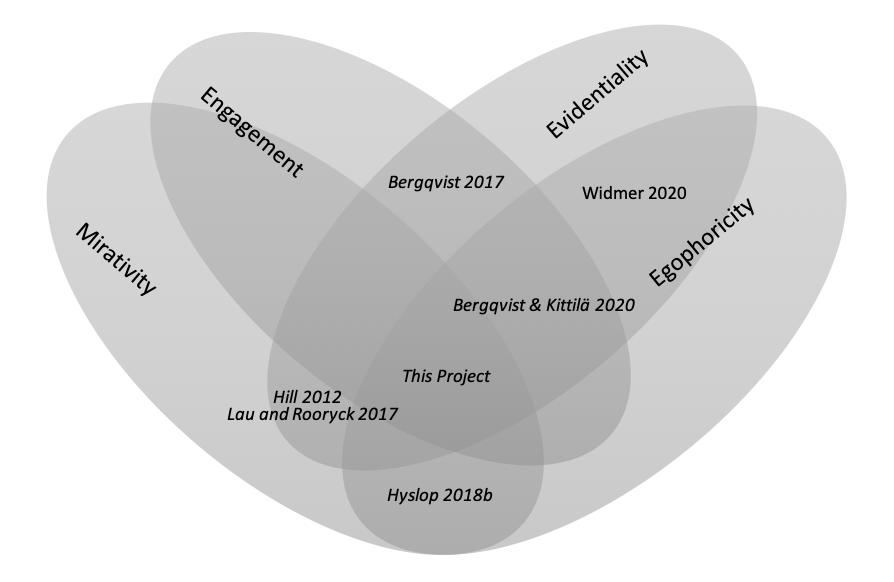
\includegraphics[width=\textwidth]{LitVenn.png}
    \caption{Examples of publications examining the crossovers between phenomena}
    \label{fig:LitVenn}
\end{figure}

\section{Paradigmatic and scattered systems}
\subsection{Paradigmatic systems}\label{sss:Discussion:Paradigmatic}
\citeA{Aikhenvald2004} refers to a type of epistemic-marking system in which various epistemic (or, in the case of \citeA{Aikhenvald2004}, evidential) bases are marked by grammatical forms across different domains of the grammar of a given language. I argue that this term of description is a gradient rather than a binary contrast. Paradigmatic systems here represent the opposite end of this gradient, in opposition to the scattered systems described by Aikhenvald. When contrasted against the alternative type of system, the intended definition of this paradigmatic category is fairly clear; however, for the purposes of this thesis, a more explicitly stated definition of the term \textsc{paradigm} is more useful. As noted above, the two categories of paradigmatic and scattered systems do not exist in a true binary, but rather can be taken to be gradual. For example, in Kurtöp (East Bodish: Bhutan) as is discussed in a case study below, the epistemic system exists across multiple domain-restricted paradigms, as well as in a small number of forms that appear to exist outside these paradigms. As such, for the most part, the epistemic system in Kurtöp appears prototypically paradigmatic, but when factoring in these few clitics that can appear across multiple grammatical domains and in combintation with the full epistemic-marking paradigms, it is not entirely so.

The term \textsc{paradigm} is widely used throughout linguistics and carries a generally accepted meaning, but specific definitions of such a basic term are harder to come by. Two levels of specificity appear to exist. On the one hand, defintions such as those in \citeA{Aronoff2023} and \citeA{Trask1993} frame the paradigm specifically as a set of inflected forms of a single stem. Others more broadly define the term as referring to any set of linguistic forms with a common property, such as, at an extreme, all nouns \cite{Booij2007}. While \citeA{Trask1993} limits his definition to the use described by \citeA{Blevins2016}, holding it as prevalent in pedagogically inclined literature, he does give a broader definition of ``paradigmatic relation.'' This he defines as ``Any relation between two or more linguistic elements which are in some sense competing possibilities, in that exactly one of them may be selected to occupy some particular position in a structure'' \cite[197]{Trask1993}. Ultimately this concept dates back to Saussure's contrast between syntagmatic and associative (or paradigmatic) relations \cite{Saussure2013}.

The definition used here exists in-between these two. Generally it refers to the set of possible inflections of a given stem as given in \citeA{Trask1993}, but skews toward to the actual inflecting morphology rather than the composed forms. In this sense, it follows the more general Saussurean concept of paradigmatic relations as defined by \citeA{Trask1993} as sets of morphemes with any functional similarities. That is, in describing a set of forms as paradigmatic rather than scattered, they are described as contributing to the set of inflected forms available for a given stem, and as having their usage conditioned by a functionally coherent and similar factors. In practice, this first trait means that the forms in a paradigmatic system will occupy the same grammatical slot---whether that be as affixal morphology, clitics, or particles---in a given location within a sentence (often final). This leads to a working definition of a set of forms that can occupy the same grammatical slot (per the pedagogical use of paradigm) and also cover a functionally coherent set of meanings (per the Saussurean concept of paradigmatic relations). This defintion is given in Figure \ref{f:Discussion:Paradigm}. One challenge with Trask's definition of paradigmatic relations, quoted above, is the necessity that these forms be mutually exclusive. In order for forms to occupy the same grammatical slot and in turn produce a neat set of inflected forms, this stipulation is understandable, but does not consistently hold across the paradigmatic systems actually seen in the data. That is, systems that otherwise appear very paradigmatic have been documented to allow cooccurrence of forms. In Eastern Geshiza \cite[rGyalrongic: PRC,][]{Honkasalo2019}, which will be discussed as case study in greater detail below, epistemic suffixes that occupy the same grammatical slot can cooccur. In these cases, the origo of the epistemic meaning is traced back along the line of sources. For instance, the cooccurrence of the sensory and reportative forms marks that the current speaker knows the given information as they heard it from another, who in turn had first hand evidence. Despite this possibility, the system is still paradigmatic in that its forms still both occupy the same grammatical slot on the verb and carry meanings within the coherent domain of epistemic meaning.

\begin{figure}
    \begin{itemize}
        \item[] \textbf{Necessary traits of a grammatical paradigm:}
        \item[+] Set of forms occupying the same grammatical slot
        \item[+] Set of functions falling under a coherent functional domain
        \item[] \textbf{Unnecessary but common traits:}
        \item[?] Forms within set are totally mutually exclusive
    \end{itemize}
    \caption{Working definition of \textsc{paradigm}.}\label{f:Discussion:Paradigm}
\end{figure}

There is a risk of a circular definition in terms of the coherent functional domain criterion. The presence of these paradigms is in part used in this thesis as proof that the meanings across these paradigms do fall into a coherent functional domain. At the same time the existence of the paradigm is defined against this coherent functional domain that is itself proven essentially by its presence across a single paradigm. This chapter aims, however, to show that this functional coherence can be seen outside of the basic fact that the forms exist in a paradigm; the same functional coherence is visible also in scattered systems. It also argues for the more general epistemic supercategory in terms beyond simple morphological structure and form.

There remains a final question of how to handle sets of forms which fulfil the first criterion, in that they occur in the same grammatical slot, but do not appear to a coherent functional domain. In Siyewu Khroskyabs \cite[rGyalrongic: PRC,][34]{TaylorAdams2020}, there is a large set of verbal prefixes that appear to occupy the same grammatical slot on the verb but which do not reflect a coherent functional domain. They are specifically described as not being in paradigmatic opposition, as they can cooccur; though, as was discussed above, this is not seen here as an excluding factor. Functionally, these forms include the negative \textit{mə-}, an interrogative \textit{(t)ɕʰə(ɣ)-}, an evidential \textit{ʐə̂-}, among nine others. Here, despite being a set of forms that occupy the same grammatical slot, the lack of any functional coherence across the set precludes them from being considered a single paradigm; a conclusion which seems to logically hold. There is an interesting example in Poumai Naga (Angami-Pochuri: India), which has a set of sentence final markers that occur after the verb in a similar formal position \cite{Veikho2021}. Functionally, two of the forms are epistemic and the other three are tense/aspect related. While in isolation they appear to occupy the same grammatical slot, an interesting pattern appears when forms are combined. Specifically, any of the three T/A markers can cooccur with either of the epistemic markers, and when they do, the T/A forms must come before the epistemic ones for the construction to be considered grammatical \cite[278]{Veikho2021}. That is, while either of the functional groups can grammatically occur in isolation, when they are combined it becomes apparent that in fact there are two different grammatical slots being filled, each of which shows a coherent functional domain and could therefore be considered a paradigm for the purposes of this analysis.

Mixed paradigmatic systems, then, are systems wherein sets of forms fulfil the criteria given in Figure \ref{f:Discussion:Paradigm}; but more specifically, wherein the coherent functional domains extend beyond a single one of the discussed traditional cross-linguistic categories. As mentioned above, the validity of describing these broader sets of functions as following a coherent functional domain is argued throughout the rest of this chapter.

\subsubsection{Scattered systems}\label{sss:Discussion:Scattered}
In the previous discussion on paradigmatic systems and the defintion of paradigm, situations discussed included a set of forms occupied a single grammatical slot but did not fall under a coherent functional domain. Scattered systems can be seen as the alternative to this, as forms do not occupy the same grammatical slot but can nonetheless be grouped according to their shared functional domain. It is argued above that the selection of forms within an epistemic system (or any set of functionally contrastive forms) is informed by an assessment of all conditioning factors relevant to the system. Part of the argument for the coherence of these sets of forms, and part of the justification for even considering them a single functional system is their functionally contrastive meanings. This is easy to see in paradigmatic systems, as forms exist contrastively both functionally and formally, in that they occupy the same grammatical slot and as such are more literally formally contrasted, even if strict mutual exclusivity is not being considered a necessary trait of a grammatical paradigm. This poses the question of whether or not this functional cohesion applies also to scattered systems, where epistemic contrasts are marked with formally disparate strategies. I argue that it does, as the functional content of the various epistemic-marking strategies in a scattered system is not inherently tied to the literal form of the marking. This is to say that, for example, a direct evidential suffix, a reportative evidential enclitic, and a non-shared information sentence-final particle are not influenced functionally---at least not in terms of their epistemic content---by their literal form. The difference in scope of, for instance, a suffix which attaches directly to the verb compared to an enclitic which attaches to a clause level, means that it would exist higher on the theoretical syntax tree that would be drawn of a speech act, creating some functional difference. It is not clear to me that this would have any impact specifically on the epistemic meaning of the forms. As such, there is no reason, especially in cases where the epistemic-marking strategies of scattered epistemic systems do not cooccur, that they should not be considered equally as functionally contrastive, and in turn part of a functionally cohesive domain as with paradigmatic systems. A speaker producing an epistemically marked speech act, whether their language has a more paradigmatic or more scattered system, still must consider every applicable conditioning factor across the possible epistemic marking for that speech act in order to select the most correct form at the exclusion of others. The necessity of this process is not dependent on the formal similarity of the epistemic marking; the meanings are contrastive and therefore exist within a cohesive system regardless. In any given speech act, the speaker (though typically not consciously) considers every available communicative tool and selects the most relevant ones. 

There is a challenge in terminology here, specifically in the use of the term `system'. Thus far, the `epistemic system' or `epistemic-marking system' has been used to refer to the whole set of grammatical epistemic-marking strategies across a language. While this generally involves specific markers, in some languages such as Milang (Siangic: India) these strategies might instead be syntactic \cite{Modi2017}, though not periphrastic or lexical, as this project is specifically limited to grammatical marking. The epistemic-marking system of a language is not necessarily a single entity per se, and there can be multiple subsystems serving different domains of the grammar of a language. This is exemplified below in Kurtöp, which shows a predominantly paradigmatic epistemic-marking system across. The overall system can be divided into a number of subsystems, each serving in this case a different tense/aspect. There is one paradigm of epistemic marking for each of the future, the imperfective, and the perfective domains. As is discussed below, these paradigms are limited to different areas of the grammar and do not interact. They also do not mark the same set of epistemic contrasts, shown in Table \ref{t:Discussion:KurtopComparison}. This is not difficult to describe with paradigmatic systems, as the so-called subsystems exist in discrete paradigms which can be described as such. With more scattered systems, however, this use of terminology is not so easy, as a domain-limited set of epistemic markers such as the various paradigms of Kurtöp would not exist in such an easily described set. This is less an issue of theory than it is one of terminology, but it remains that a term is needed to describe domain-restricted sets of scattered epistemic markers below the level of the system. Other literature has already used the term `subsystem', namely \citeA{Aikhenvald2004}, and as such the term will also be used here.

\section{Theoretical approaches to speech act construction}\label{ss:Discussion:SpeechActs}
Much of the analysis throughout this thesis, particularly in \cref{c:Discussion}, discusses the internal process of constructing a speech act in a theoretical sense. I do not intend here to make any claims regarding psycholinguistics or neurology in terms of the actual mechanisms by which language is developed and constructed in the brain, but rather to speak theoretically about the decision-making process in choosing one specific form over another. While this process of form selection is clearly rarely if never a conscious one, it appears to be particularly subconscious in the case of epistemic distinctions. \citeA{Grzech2020} note that the exact rules around the usage of epistemic forms in language are not reliably consciously available to speakers, as will be discussed in \appref{s:Methods:FieldMethods} with regards to the field work undertaken on Lhokpu as part of this project. Whether conscious or not, however, there is necessarily still some process by which forms are chosen as language is constructed. This discussion provides a foundation for the analysis and subsequent arguments presented in \cref{c:Discussion} discussing the selection of forms in speech act construction and the implication this has for the prevalence of attention to perspective in speech more generally.

There are two general conceptualisations of this process that will be used in the following analysis. The first is a sort of bottom-up approach in which a form is selected for its given meaning. That is, a speaker is attempting to communicate some meaning \textit{xyz}, and as such selects forms with meaning \textit{x, y} and \textit{z}. This, of course, is greatly simplified, and does not account for, for instance, agreement, in which multiple forms in a given speech act carry the same meaning. The essence of the conceptualisation is, in any case, that in order to communicate a given meaning, the speaker will select forms with the necessary component meanings for successful communication. The second conceptualisation, on the other hand, views the meanings of individual forms as being comprised of a series of conditions that need to be met in order for that form to be used. In selecting a given form the speaker considers these conditions against the conditions of the speech act---being both the propositional content of the speech act and its deictic context---and subsequently selects the forms whose conditions have been met. Here, if a speaker is trying to communicate \textit{abc}, they might, for example, consider a set or paradigm of forms with the conditions of \textit{c, d, e,} and \textit{f}. In choosing the form \textit{c}, the speaker considers each form against their intended \textit{abc} to see which best fits, and as such, also considers whatever conditions \textit{d, e,} and \textit{f} represent along with the actually applicable \textit{c}. This is particularly abstract without a concrete example, though it forms a basis for the case studies presented in Section \ref{ss:Discussion:MixedCases}, where it is exemplified more clearly. The primary difference between these conceptualisations is in how much the speaker is explicitly seen to consider when selecting a form. That is, in the first conceptualisation, the speaker only considers the meaning they wish to communicate, whereas in the second, the speaker is also necessarily considering conditions which are not necessarily relevant to their intended meaning. This wider consideration implied in the second conceptualisation serves the purpose of selecting a given form in opposition to similar ones, such as contrasting forms in a single paradigm. Additionally, it is easier to ascribe multiple conditions to an epistemic form where only one would be considered the primary meaning. This process would still be theoretically present in any case regardless of the conceptualisation through which the selection of forms is being described. In essence, the two methods used in the following analyses of describing forms, their meanings, and the processes around how they are selected, are not intended to be seen as two different processes; rather, they are two ways of describing or conceptualising the cognitive communicative process.